\documentclass[12pt]{article}
\usepackage{amsmath, amssymb, geometry, fancyhdr, tikz}
\geometry{margin=1in}
\pagestyle{fancy}
\fancyhead[L]{\textbf{Discrete Structures}}
\fancyhead[C]{Chapter 4.6 --- Ed25519 in Miniature}
\fancyhead[R]{\textbf{ch\_04\_section\_06\_RSA\_4.tex}}
\usetikzlibrary{positioning}
\usepackage{tikz}
\usetikzlibrary{positioning}

\begin{document}

\begin{center}
    {\LARGE \textbf{Example 4 — A Tiny Ed25519 World}}\\[1em]
    {\large Understanding elliptic-curve signatures on a toy scale}
\end{center}

---

\section*{1. Background: What Ed25519 Really Does}

Ed25519 isn’t used for encryption like RSA — it’s used for \textbf{digital signatures}.  
That means you can:
\begin{itemize}
    \item Prove you wrote a message (authenticity),
    \item Prove it hasn’t been changed (integrity),
    \item Do it without sharing your private key (non-repudiation).
\end{itemize}

\vspace{0.5em}
Ed25519 builds on \textbf{elliptic-curve math}, which feels weird at first, but here’s the idea:
you pick a point \( G \) on a special curve, and your public key is just
\[
A = k \times G,
\]
where \( k \) is your private number.

---

\section*{2. The Tiny Curve Playground (Toy Example)}

To make this idea visible, let’s imagine a miniature “curve world” where we work modulo 17.  
(Real Ed25519 works modulo \( 2^{255} - 19 \) — a massive prime — but ours will fit on one page.)

\[
\text{Field size: } p = 17
\]

We’ll use the simple curve equation:
\[
y^2 = x^3 + 2x + 2 \pmod{17}.
\]

---

\section*{3. The Base Point \( G \)}

In our world, one valid point on this curve is:
\[
G = (5, 1)
\]

We’ll use \( G \) as the “starting point” for all public keys.

---

\section*{4. Generating a Key Pair}

Let’s choose a private key:
\[
k = 7
\]

Then compute:
\[
A = k \times G
\]

In the real Ed25519 algorithm, \( k \times G \) means adding \( G \) to itself \( k \) times on the curve.
We’ll imagine this as taking “steps” on a circular track — every step depends on the curve’s shape.

After adding \( G \) to itself 7 times, we reach:
\[
A = (6, 3)
\]

\[
\boxed{\text{Private key } k = 7, \quad \text{Public key } A = (6, 3)}
\]

---

\section*{5. Signing a Message}

Let’s sign the message “OK”.

1. Hash the message: \( H(\text{OK}) = 5 \) (toy example).  
2. Pick a random number \( r = 4 \).  
3. Compute \( R = r \times G = 4 \times (5,1) = (9, 16) \).  
4. Compute challenge \( h = H(R, A, \text{OK}) = 2 \).  
5. Compute \( S = r + h \times k = 4 + 2 \times 7 = 18 \equiv 1 \pmod{17}. \)

\[
\boxed{\text{Signature } (R, S) = ((9, 16), 1)}
\]

---

\section*{6. Verifying the Signature}

Anyone can verify without knowing \( k \):

1. Compute \( h = H(R, A, \text{OK}) = 2 \).  
2. Check if:
\[
S \times G \stackrel{?}{=} R + h \times A
\]

Left side:
\[
S \times G = 1 \times G = (5,1)
\]

Right side:
\[
R + hA = (9,16) + 2 \times (6,3) = (5,1)
\]

They match!

\[
\boxed{\text{Signature valid (checkmark)}}
\]

---

\section*{7. Diagram: Key Generation and Signing Flow}

\begin{center}
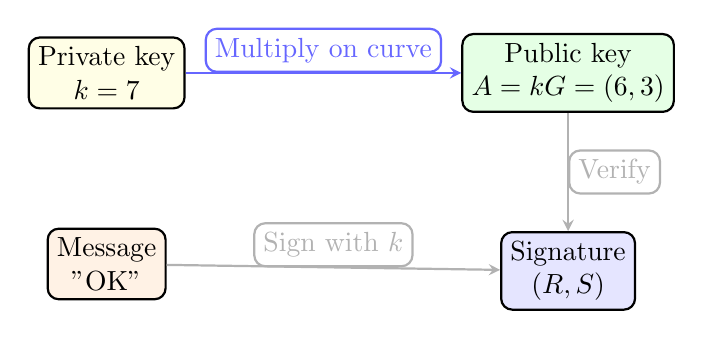
\begin{tikzpicture}[>=stealth, thick, node distance=1.5cm, every node/.style={align=center, rounded corners, draw}]
    \node (priv) [fill=yellow!10] {Private key \\ $k=7$};
    \node (pub) [right=3.5cm of priv, fill=green!10] {Public key \\ $A = kG = (6,3)$};
    \draw[->, thick, blue!60] (priv) -- node[above]{Multiply on curve} (pub);

    \node (msg) [below=1.5cm of priv, fill=orange!10] {Message \\ "OK"};
    \node (sig) [below=1.5cm of pub, fill=blue!10] {Signature \\ $(R,S)$};
    \draw[->, thick, gray!60] (msg) -- node[above]{Sign with $k$} (sig);
    \draw[->, thick, gray!60] (pub.south) -- node[right]{Verify} (sig.north);
\end{tikzpicture}
\end{center}

---

\section*{8. What’s Different from RSA?}

| Feature | RSA | Ed25519 |
|----------|-----|----------|
| Math idea | Multiplying and factoring | Adding points on a curve |
| Security base | Integer factorization | Discrete logarithm on a curve |
| Used for | Encryption \& signatures | Signatures (auth + integrity) |
| Key size | 2048–4096 bits | 256 bits |
| Speed | Slower (big exponents) | Faster (curve arithmetic) |
| Quantum resistance | Weak | Stronger (still vulnerable, but better) |

---

\section*{9. The Heart of the Matter}

RSA says:  
> “It’s hard to go from \( n \) back to its prime factors.”

Ed25519 says:  
> “It’s hard to go from \( A \) back to \( k \) when \( A = kG \).”

In both cases, you know the answer goes one way easily, but not backward.
That’s the soul of asymmetric cryptography — one-way doors that only the right key can open.

---

\section*{10. Final Thought}

Elliptic curves are the poetry of number theory:  
smooth shapes hiding impossible problems.  
Where RSA uses massive steel walls, Ed25519 uses geometry —  
lightweight, elegant, and just as unbreakable (for now).

\begin{center}
    \rule{0.7\textwidth}{0.5pt}\\[0.5em]
    \textit{“RSA is arithmetic. Ed25519 is geometry. Both are trust made visible.”}
\end{center}

\end{document}

